\documentclass[14pt,a4paper]{extarticle}

% Компилятор: XeLaTeX. Для minted требуется параметр -shell-escape.
\usepackage{fontspec}
\usepackage{polyglossia}
\setdefaultlanguage{russian}

\IfFontExistsTF{Liberation Serif}
    {\setmainfont{Liberation Serif}}
    {\setmainfont{FreeSerif}}
\IfFontExistsTF{DejaVu Sans Mono}
    {\setmonofont{DejaVu Sans Mono}}
    {\setmonofont{FreeMono}}

\usepackage[left=30mm,right=15mm,top=20mm,bottom=20mm]{geometry}
\usepackage{setspace}
\onehalfspacing
\setlength{\parindent}{1.25cm}
\setlength{\parskip}{0pt}
\setlength{\emergencystretch}{3em}

\usepackage{microtype}
\usepackage{ragged2e}
\usepackage{enumitem}
\usepackage{titlesec}
\usepackage{tocloft}
\usepackage{longtable}
\usepackage{tabularx}
\usepackage{array}
\usepackage{booktabs}
\usepackage{float}
\usepackage{amsmath}
\usepackage{xcolor}
\usepackage{minted}
\usepackage{graphicx}
\usepackage{pdflscape}
\usepackage{adjustbox}
\usepackage{tikz}
\usetikzlibrary{arrows.meta,positioning,shapes.geometric,fit,calc}
\usepackage[hidelinks]{hyperref}

\titleformat{\section}
    {\bfseries\fontsize{14pt}{17pt}\selectfont}
    {\thesection}{0.8em}{}
\titleformat{\subsection}
    {\bfseries\fontsize{14pt}{17pt}\selectfont}
    {\thesubsection}{0.8em}{}
\titlespacing*{\section}{0pt}{12pt}{12pt}
\titlespacing*{\subsection}{0pt}{12pt}{6pt}

\renewcommand{\contentsname}{СОДЕРЖАНИЕ}
\setlength{\cftbeforesecskip}{0pt}
\setlength{\cftbeforesubsecskip}{0pt}

\definecolor{CodeBackground}{RGB}{247,247,247}
\definecolor{EntityBlue}{RGB}{224,238,249}
\definecolor{EntityGreen}{RGB}{226,242,226}
\definecolor{EntityOrange}{RGB}{252,235,215}

\setminted{
    fontsize=\small,
    breaklines=true,
    linenos=true,
    numbersep=7pt,
    frame=single,
    framesep=3mm,
    bgcolor=CodeBackground,
    tabsize=4,
    autogobble=true
}

\newcolumntype{Y}{>{\RaggedRight\arraybackslash}X}
\newcolumntype{L}[1]{>{\RaggedRight\arraybackslash}p{#1}}

% Скриншоты интерфейса можно добавить позднее в report/images.
% Если файла нет, отчёт остаётся корректным и выводит текстовое примечание.
\newcommand{\optionalinterfacefigure}[2]{%
    \IfFileExists{images/#1.png}{%
        \begin{figure}[H]
            \centering
            \includegraphics[width=0.94\textwidth,height=0.58\textheight,keepaspectratio]{images/#1.png}
            \caption{#2}
            \label{fig:#1}
        \end{figure}
    }{%
        \begin{center}
            \fbox{\parbox{0.88\textwidth}{\centering
                Место для скриншота «#2».\\
                Имя файла: \nolinkurl{images/#1.png}}}
        \end{center}
    }%
}

\newcommand{\StudentGroup}{421702}
\newcommand{\StudentName}{А.\,В.~Сайковский}
\newcommand{\TeacherName}{Н.\,А.~Гуменный}
\newcommand{\VariantNumber}{23}

\begin{document}
\justifying
\pagestyle{plain}

% ============================================================================
% 1. ТИТУЛЬНЫЙ ЛИСТ
% ============================================================================
\begin{titlepage}
\thispagestyle{empty}
\begin{center}
Министерство образования Республики Беларусь

Учреждение образования

\vspace{0.2cm}

\textbf{БЕЛОРУССКИЙ ГОСУДАРСТВЕННЫЙ УНИВЕРСИТЕТ}\\
\textbf{ИНФОРМАТИКИ И РАДИОЭЛЕКТРОНИКИ}

\vspace{0.3cm}

Факультет информационных технологий и управления

Кафедра интеллектуальных информационных технологий

\vfill

{\Large\textbf{ОТЧЁТ}}

\vspace{0.4cm}

о выполнении лабораторной работы №2

по дисциплине «Проектирование баз знаний»

\vspace{0.4cm}

на тему:

\vspace{0.3cm}

{\large\textbf{Проектирование и разработка информационной системы\\
«Банк данных технологий создания продуктов»}}

\vspace{0.3cm}

(Вариант №\VariantNumber)

\vfill
\end{center}

\begin{flushright}
\begin{minipage}{0.48\textwidth}
Студент гр. \StudentGroup

\StudentName

\vspace{0.6cm}

Преподаватель

\TeacherName
\end{minipage}
\end{flushright}

\vfill

\begin{center}
Минск 2026
\end{center}
\end{titlepage}

% ============================================================================
% 2. СОДЕРЖАНИЕ
% ============================================================================
\setcounter{page}{1}
\clearpage
\tableofcontents

% ============================================================================
% 3. ПОСТАНОВКА ЗАДАЧИ
% ============================================================================
\clearpage
\section{ПОСТАНОВКА ЗАДАЧИ}

\subsection{Описание предметной области}

Предметной областью разрабатываемой информационной системы является учёт
технологий производства пищевых продуктов. Производственное предприятие
выпускает товары разных групп: хлебобулочные, кондитерские и молочные изделия,
напитки, соусы и другие виды продукции. Для каждого товара может существовать
один или несколько рецептов. Рецепт имеет уникальный номер, название,
текстовое описание и автора.

Состав рецепта определяется перечнем ингредиентов. Для каждого ингредиента в
конкретном рецепте необходимо знать его массу в граммах на один килограмм
готового продукта и способ подготовки: просеивание, нагревание, смешивание,
взбивание и т.~д. Один ингредиент может входить во многие рецепты, а один
рецепт состоит из многих ингредиентов. Калорийность готового продукта
рассчитывается на основании калорийности и массы составляющих.

Ингредиенты приобретаются у поставщиков. Факт поставки оформляется накладной,
которая содержит поставщика, номер и дату. Каждая позиция накладной указывает
ингредиент, поставленное количество и цену единицы. Один поставщик может
оформить множество накладных, а одна накладная содержит множество позиций.

Система должна обеспечивать централизованное хранение данных, соблюдение
ссылочной целостности, просмотр и изменение записей через web-интерфейс, а
также формирование аналитических отчётов.

\subsection{Функциональные требования}

Пользователь должен иметь возможность:

\begin{enumerate}[leftmargin=1.25cm]
    \item просматривать, добавлять, изменять и удалять товары;
    \item вести справочники групп товаров и способов подготовки;
    \item вести сведения об ингредиентах и их калорийности;
    \item вести сведения об авторах и рецептах;
    \item вести сведения о поставщиках и накладных;
    \item получать прайс-лист поставщика на выбранную дату;
    \item определять товары с минимальной калорийностью;
    \item получать список товаров и связанных с ними рецептов.
\end{enumerate}

\subsection{Нефункциональные требования}

Приложение должно работать асинхронно, проверять входные данные, использовать
PostgreSQL и ручные параметризованные SQL-запросы. Значения, введённые во
frontend, не должны объединяться со строкой SQL. Ошибки целостности должны
приводить к откату транзакции и понятному HTTP-ответу. База данных должна
запускаться воспроизводимо через Docker Compose, а основные операции должны
быть покрыты автоматическими тестами.

% ============================================================================
% 4. КОНЦЕПТУАЛЬНОЕ ПРОЕКТИРОВАНИЕ
% ============================================================================
\clearpage
\section{КОНЦЕПТУАЛЬНОЕ ПРОЕКТИРОВАНИЕ}

Для описания поведения системы выбрана диаграмма вариантов использования
(Use Case). Основным актором является пользователь приложения --- сотрудник,
который ведёт технологические и закупочные данные. Диаграмма представлена на
рисунке~\ref{fig:usecase}.

\iffalse
\begin{figure}[H]
\centering
\begin{tikzpicture}[
    font=\small,
    actor/.style={draw,circle,minimum size=7mm,inner sep=0pt},
    usecase/.style={draw,ellipse,minimum width=5.0cm,minimum height=1.15cm,align=center,fill=EntityBlue},
    relation/.style={thick},
    include/.style={-{Latex[length=2.5mm]},dashed}
]
% Актор
\node[actor] (head) at (-6,1.6) {};
\draw (-6,1.25) -- (-6,0.15);
\draw (-6,0.95) -- (-6.65,0.45);
\draw (-6,0.95) -- (-5.35,0.45);
\draw (-6,0.15) -- (-6.6,-0.65);
\draw (-6,0.15) -- (-5.4,-0.65);
\node[align=center] at (-6,-1.15) {Пользователь};

% Граница системы
\node[draw,minimum width=11.7cm,minimum height=12.2cm,anchor=north west] (system) at (-3.8,5.4) {};
\node[anchor=north west,font=\bfseries] at (-3.55,5.2) {Информационная система};

% Варианты использования
\node[usecase] (dict) at (-0.7,3.8) {Вести справочники};
\node[usecase] (products) at (-0.7,1.9) {Управлять товарами};
\node[usecase] (recipes) at (-0.7,0.0) {Управлять рецептами};
\node[usecase] (suppliers) at (-0.7,-1.9) {Управлять поставщиками};
\node[usecase] (invoices) at (-0.7,-3.8) {Управлять накладными};
\node[usecase,fill=EntityGreen] (price) at (4.1,2.8) {Получить прайс-лист\\поставщика};
\node[usecase,fill=EntityGreen] (calories) at (4.1,0.5) {Найти товары с минимальной\\калорийностью};
\node[usecase,fill=EntityGreen] (productrecipes) at (4.1,-1.8) {Получить товары\\с рецептами};
\node[usecase,fill=EntityOrange,minimum width=4.2cm] (validate) at (4.1,-4.0) {Проверить данные};

% Связи актора
\foreach \target in {dict,products,recipes,suppliers,invoices,price,calories,productrecipes}
    \draw[relation] (-5.35,0.75) -- (\target.west);

% Include
\draw[include] (products.east) -- node[above,sloped]{\scriptsize <<include>>} (validate.north);
\draw[include] (recipes.east) -- node[above,sloped]{\scriptsize <<include>>} (validate.north west);
\draw[include] (invoices.east) -- node[below,sloped]{\scriptsize <<include>>} (validate.west);
\end{tikzpicture}
\caption{Диаграмма вариантов использования системы}
\label{fig:usecase}
\end{figure}
\fi

\begin{figure}[H]
\centering
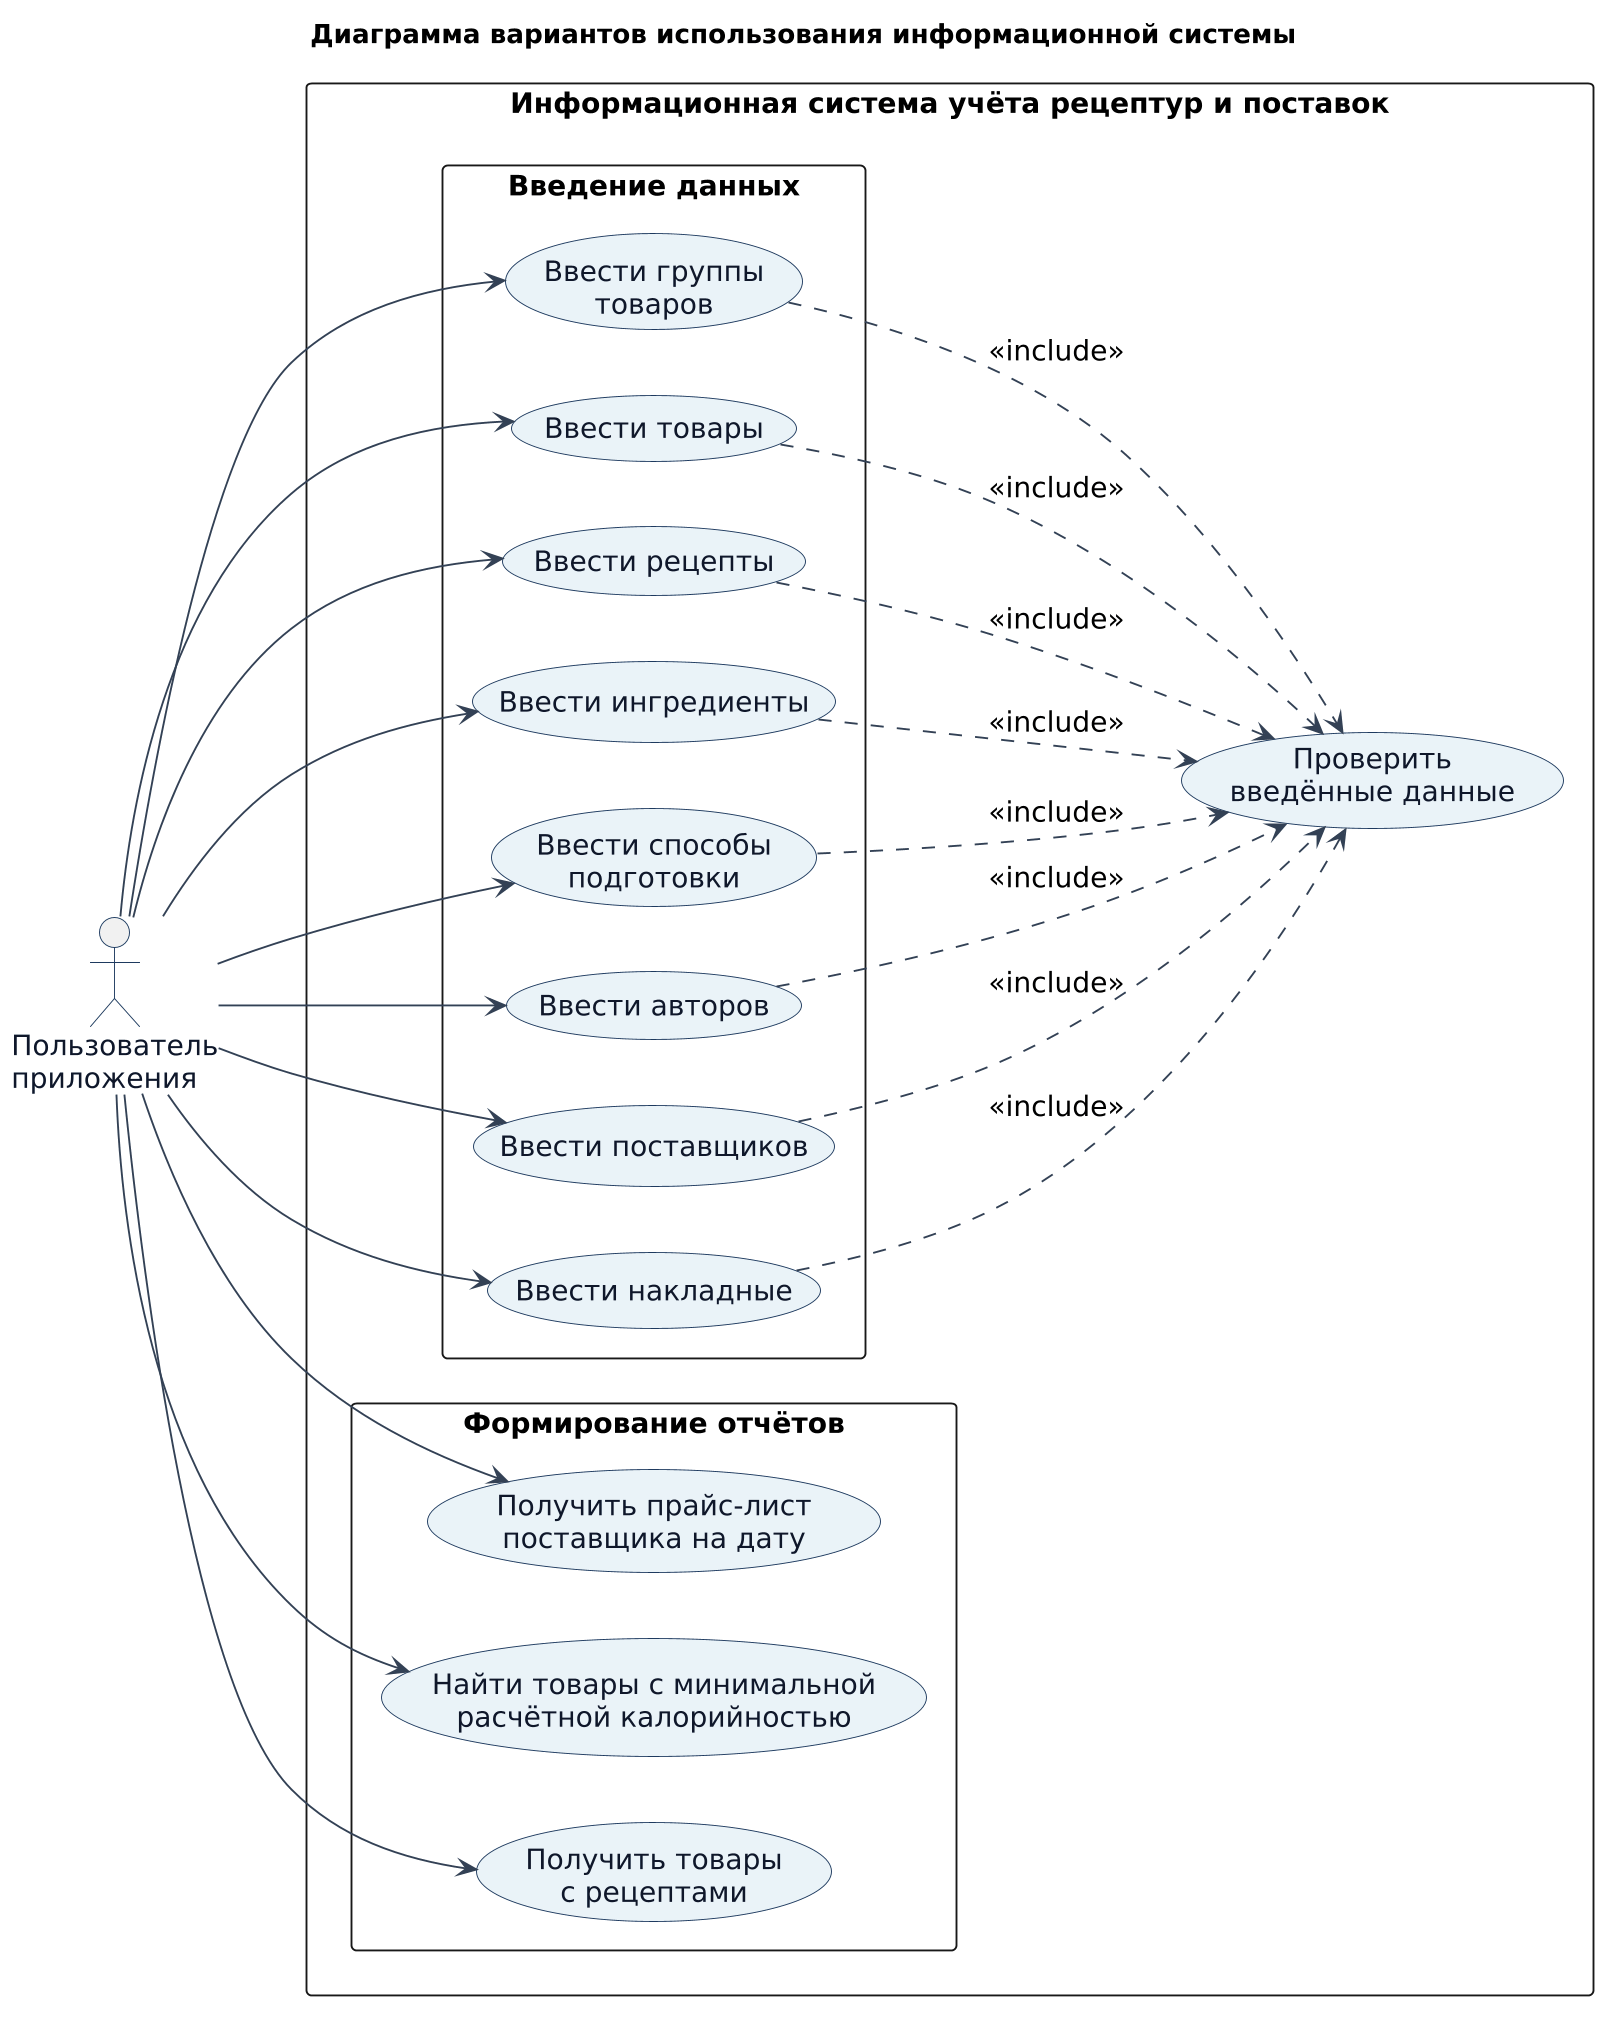
\includegraphics[width=0.92\textwidth,height=0.72\textheight,keepaspectratio]{images/01_use_case.png}
\caption{Диаграмма вариантов использования системы}
\label{fig:usecase}
\end{figure}

\subsection{Спецификация ВИ-01 «Управлять записями»}

\begin{longtable}{L{0.25\textwidth} L{0.65\textwidth}}
\toprule
\textbf{Поле} & \textbf{Описание} \\
\midrule
\endhead
Идентификатор & ВИ-01. \\
Цель & Создать, просмотреть, изменить или удалить запись выбранного ресурса. \\
Актор & Пользователь. \\
Предусловия & Приложение запущено; соединение с базой данных установлено. \\
Основной сценарий & 1) Пользователь открывает раздел. 2) Система загружает список. 3) Пользователь выбирает действие и вводит данные. 4) Система проверяет данные. 5) Выполняется параметризованный SQL-запрос. 6) Транзакция фиксируется. 7) Обновлённый список выводится на экран. \\
Альтернативы & Неверные данные --- HTTP 422; запись не найдена --- HTTP 404; нарушено ограничение БД --- HTTP 409 с откатом транзакции. \\
Постусловия & База данных изменена только при успешном завершении операции. \\
\bottomrule
\end{longtable}

\subsection{Спецификация ВИ-02 «Получить прайс-лист поставщика»}

\begin{longtable}{L{0.25\textwidth} L{0.65\textwidth}}
\toprule
\textbf{Поле} & \textbf{Описание} \\
\midrule
\endhead
Идентификатор & ВИ-02. \\
Цель & Получить цены ингредиентов определённого поставщика на выбранную дату. \\
Актор & Пользователь. \\
Предусловия & Поставщик зарегистрирован в системе. \\
Основной сценарий & 1) Пользователь задаёт поставщика и дату. 2) Система проверяет существование поставщика. 3) Выполняется соединение накладных, позиций и ингредиентов. 4) Возвращаются наименования, цены и номера накладных. \\
Альтернативы & Поставщик отсутствует --- HTTP 404; поставки на дату отсутствуют --- возвращается пустой список позиций. \\
Постусловия & Данные не изменяются. \\
\bottomrule
\end{longtable}

\subsection{Спецификация ВИ-03 «Найти товары с минимальной калорийностью»}

\begin{longtable}{L{0.25\textwidth} L{0.65\textwidth}}
\toprule
\textbf{Поле} & \textbf{Описание} \\
\midrule
\endhead
Идентификатор & ВИ-03. \\
Цель & Определить рецепты с наименьшей расчётной калорийностью. \\
Актор & Пользователь. \\
Предусловия & В БД присутствуют рецепты и их компоненты. \\
Основной сценарий & 1) Пользователь запускает отчёт. 2) Для каждого рецепта суммируются произведения массы и калорийности ингредиентов. 3) Определяется минимум. 4) Система возвращает все рецепты с минимальным значением. \\
Альтернативы & Рецепты с компонентами отсутствуют --- минимум равен нулю, список пуст. \\
Постусловия & Данные не изменяются. \\
\bottomrule
\end{longtable}

\subsection{Спецификация ВИ-04 «Получить товары с рецептами»}

\begin{longtable}{L{0.25\textwidth} L{0.65\textwidth}}
\toprule
\textbf{Поле} & \textbf{Описание} \\
\midrule
\endhead
Идентификатор & ВИ-04. \\
Цель & Получить иерархический перечень товаров и вариантов их рецептов. \\
Актор & Пользователь. \\
Предусловия & В системе зарегистрированы товары и рецепты. \\
Основной сценарий & 1) Пользователь открывает отчёт. 2) Система соединяет товары, группы и рецепты. 3) Строки группируются по товару. 4) Возвращается JSON со списком рецептов внутри каждого товара. \\
Альтернативы & Подходящие записи отсутствуют --- возвращается пустой список. \\
Постусловия & Данные не изменяются. \\
\bottomrule
\end{longtable}

% ============================================================================
% 5. ЛОГИЧЕСКОЕ ПРОЕКТИРОВАНИЕ
% ============================================================================
\clearpage
\begin{landscape}
\section{ЛОГИЧЕСКОЕ ПРОЕКТИРОВАНИЕ}

Логическая модель содержит основные сущности предметной области, их атрибуты
и мощности связей, но не зависит от конкретных типов PostgreSQL. ER-диаграмма
приведена на рисунке~\ref{fig:er}.

\iffalse
\begin{figure}[H]
\centering
\begin{tikzpicture}[
    font=\small,
    entity/.style={rectangle,rounded corners,draw,thick,minimum width=3.8cm,minimum height=1.15cm,align=center,fill=EntityBlue},
    assoc/.style={rectangle,draw,thick,minimum width=4.5cm,minimum height=1.15cm,align=center,fill=EntityOrange},
    rel/.style={thick},
    node distance=1.8cm and 2.1cm
]
\node[entity] (group) {Группа товаров};
\node[entity,right=of group] (product) {Товар};
\node[entity,right=of product] (recipe) {Рецепт};
\node[entity,above=of recipe] (author) {Автор};
\node[assoc,right=of recipe] (ri) {Состав рецепта\\масса на 1 кг};
\node[entity,right=of ri] (ingredient) {Ингредиент\\калорийность};
\node[entity,above=of ri] (method) {Способ подготовки};
\node[entity,below=3.0cm of product] (supplier) {Поставщик};
\node[entity,right=of supplier] (invoice) {Накладная};
\node[assoc,right=of invoice] (ii) {Позиция накладной\\количество, цена};

\draw[rel] (group) -- node[above]{1} node[below]{N} (product);
\draw[rel] (product) -- node[above]{1} node[below]{N} (recipe);
\draw[rel] (author) -- node[left]{1} node[right]{N} (recipe);
\draw[rel] (recipe) -- node[above]{1} node[below]{N} (ri);
\draw[rel] (ri) -- node[above]{N} node[below]{1} (ingredient);
\draw[rel] (method) -- node[left]{1} node[right]{N} (ri);
\draw[rel] (supplier) -- node[above]{1} node[below]{N} (invoice);
\draw[rel] (invoice) -- node[above]{1} node[below]{N} (ii);
\draw[rel] (ii.east) -| node[pos=0.2,below]{N} node[pos=0.85,right]{1} (ingredient.south);
\end{tikzpicture}
\caption{Логическая ER-диаграмма предметной области}
\label{fig:er}
\end{figure}
\fi

\begin{figure}[H]
\centering
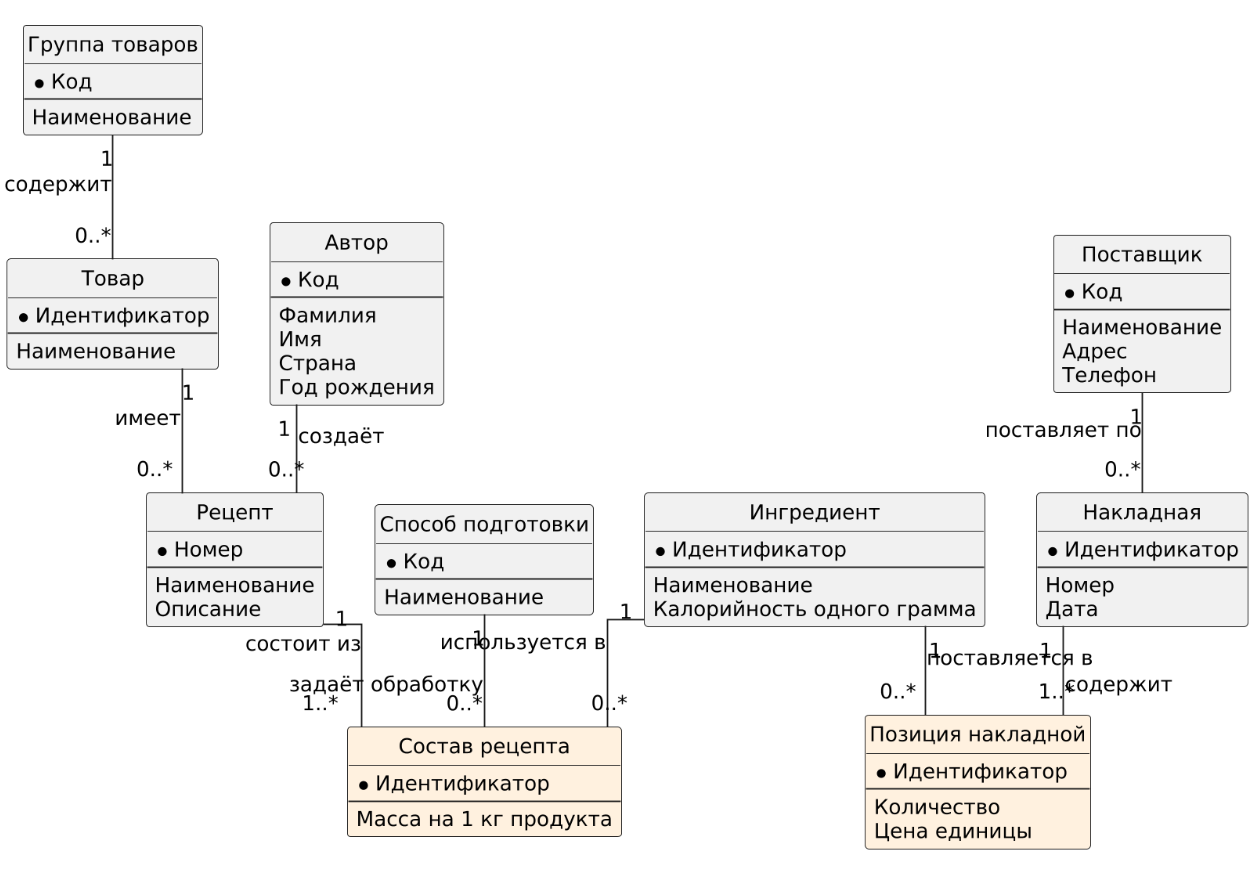
\includegraphics[width=0.96\linewidth,height=0.72\textheight,keepaspectratio]{images/02_logical_er.png}
\caption{Логическая ER-диаграмма предметной области}
\label{fig:er}
\end{figure}
\end{landscape}

\subsection{Описание сущностей}

\begin{longtable}{L{0.28\textwidth} L{0.62\textwidth}}
\toprule
\textbf{Сущность} & \textbf{Назначение и основные атрибуты} \\
\midrule
\endhead
Группа товаров & Код и наименование категории продукции. \\
Товар & Наименование производимого продукта и ссылка на группу. \\
Автор & Код, фамилия, имя, страна и год рождения автора рецепта. \\
Рецепт & Уникальный номер, название, описание, товар и автор. \\
Ингредиент & Уникальное наименование и калорийность одного грамма. \\
Способ подготовки & Код и наименование технологической операции. \\
Состав рецепта & Связь рецепта, ингредиента и способа подготовки; количество граммов на килограмм. \\
Поставщик & Код, наименование, адрес и телефон. \\
Накладная & Поставщик, номер документа и дата поставки. \\
Позиция накладной & Ингредиент, количество и цена единицы. \\
\bottomrule
\end{longtable}

\subsection{Связи и правила удаления}

\begin{longtable}{L{0.25\textwidth} L{0.18\textwidth} L{0.25\textwidth} L{0.20\textwidth}}
\toprule
\textbf{Родитель} & \textbf{Мощность} & \textbf{Дочерняя сущность} & \textbf{Правило} \\
\midrule
\endhead
Группа товаров & 1:N & Товар & RESTRICT \\
Товар & 1:N & Рецепт & CASCADE \\
Автор & 1:N & Рецепт & RESTRICT \\
Рецепт & 1:N & Состав рецепта & CASCADE \\
Ингредиент & 1:N & Состав рецепта & RESTRICT \\
Способ подготовки & 1:N & Состав рецепта & RESTRICT \\
Поставщик & 1:N & Накладная & RESTRICT \\
Накладная & 1:N & Позиция накладной & CASCADE \\
Ингредиент & 1:N & Позиция накладной & RESTRICT \\
\bottomrule
\end{longtable}

\texttt{CASCADE} используется для зависимых записей, которые не имеют смысла
без владельца. \texttt{RESTRICT} запрещает удаление справочной записи, если на
неё уже ссылаются бизнес-данные.

% ============================================================================
% 6. ФИЗИЧЕСКОЕ ПРОЕКТИРОВАНИЕ
% ============================================================================
\clearpage
\begin{landscape}
\section{ФИЗИЧЕСКОЕ ПРОЕКТИРОВАНИЕ}

\iffalse
Физическая модель ориентирована на PostgreSQL. Все таблицы имеют surrogate
primary key \texttt{id} типа \texttt{SERIAL}. Денежные, количественные и
калорийные значения хранятся в \texttt{NUMERIC}, чтобы исключить ошибки
двоичной арифметики с плавающей точкой. Схема представлена на
рисунке~\ref{fig:physical}.
\fi

\iffalse
\begin{figure}[H]
\centering
\begin{adjustbox}{max width=0.97\linewidth,max height=0.82\textheight}
\begin{tikzpicture}[
    font=\scriptsize,
    table/.style={rectangle,draw,thick,rounded corners=1pt,align=left,inner sep=5pt,fill=white},
    fk/.style={-{Latex[length=2mm]},thick},
    node distance=1.0cm and 1.5cm
]
\node[table,fill=EntityBlue] (groups) {\textbf{product\_groups}\\[-1mm]\rule{3.7cm}{0.4pt}\\
PK id SERIAL\\code VARCHAR(32) UNIQUE NOT NULL\\name VARCHAR(255) NOT NULL};

\node[table,fill=EntityBlue,below=of groups] (products) {\textbf{products}\\[-1mm]\rule{3.7cm}{0.4pt}\\
PK id SERIAL\\name VARCHAR(255) NOT NULL\\FK group\_id INTEGER NOT NULL};

\node[table,fill=EntityBlue,below=of products] (recipes) {\textbf{recipes}\\[-1mm]\rule{4.3cm}{0.4pt}\\
PK id SERIAL\\number VARCHAR(64) UNIQUE NOT NULL\\name VARCHAR(255) NOT NULL\\description TEXT\\FK product\_id INTEGER NOT NULL\\FK author\_id INTEGER NOT NULL};

\node[table,fill=EntityGreen,right=of groups] (authors) {\textbf{authors}\\[-1mm]\rule{4.3cm}{0.4pt}\\
PK id SERIAL\\code VARCHAR(32) UNIQUE NOT NULL\\surname VARCHAR(255) NOT NULL\\name VARCHAR(255) NOT NULL\\country VARCHAR(255) NOT NULL\\year INTEGER NOT NULL};

\node[table,fill=EntityOrange,right=of recipes] (ri) {\textbf{recipe\_ingredients}\\[-1mm]\rule{5.4cm}{0.4pt}\\
PK id SERIAL\\FK recipe\_id INTEGER NOT NULL\\FK ingredient\_id INTEGER NOT NULL\\FK preparation\_method\_id INTEGER NOT NULL\\grams\_per\_kg NUMERIC(12,3) NOT NULL\\UNIQUE(recipe, ingredient, method)};

\node[table,fill=EntityGreen,above=of ri] (methods) {\textbf{preparation\_methods}\\[-1mm]\rule{4.6cm}{0.4pt}\\
PK id SERIAL\\code VARCHAR(32) UNIQUE NOT NULL\\name VARCHAR(255) NOT NULL};

\node[table,fill=EntityGreen,right=of ri] (ingredients) {\textbf{ingredients}\\[-1mm]\rule{5.0cm}{0.4pt}\\
PK id SERIAL\\name VARCHAR(255) UNIQUE NOT NULL\\calories\_per\_gram NUMERIC(12,4) NOT NULL\\CHECK(calories\_per\_gram $\geq$ 0)};

\node[table,fill=EntityBlue,above=of ingredients] (suppliers) {\textbf{suppliers}\\[-1mm]\rule{4.0cm}{0.4pt}\\
PK id SERIAL\\code VARCHAR(32) UNIQUE NOT NULL\\name VARCHAR(255) NOT NULL\\address VARCHAR(255)\\phone VARCHAR(32)};

\node[table,fill=EntityBlue,right=of suppliers] (invoices) {\textbf{invoices}\\[-1mm]\rule{4.2cm}{0.4pt}\\
PK id SERIAL\\FK supplier\_id INTEGER NOT NULL\\number VARCHAR(64)\\invoice\_date DATE NOT NULL\\UNIQUE(supplier\_id, number)};

\node[table,fill=EntityOrange,below=of invoices] (items) {\textbf{invoice\_items}\\[-1mm]\rule{5.2cm}{0.4pt}\\
PK id SERIAL\\FK invoice\_id INTEGER NOT NULL\\FK ingredient\_id INTEGER NOT NULL\\quantity NUMERIC(14,3) NOT NULL\\unit\_price NUMERIC(14,4) NOT NULL\\CHECK(quantity $>$ 0)\\CHECK(unit\_price $>$ 0)\\UNIQUE(invoice\_id, ingredient\_id)};

\draw[fk] (products.north) -- (groups.south);
\draw[fk] (recipes.north) -- (products.south);
\draw[fk] (recipes.east) -| (authors.south);
\draw[fk] (ri.west) -- (recipes.east);
\draw[fk] (ri.north) -- (methods.south);
\draw[fk] (ri.east) -- (ingredients.west);
\draw[fk] (invoices.west) -- (suppliers.east);
\draw[fk] (items.north) -- (invoices.south);
\draw[fk] (items.west) -| (ingredients.east);
\end{tikzpicture}
\end{adjustbox}
\caption{Физическая схема базы данных PostgreSQL}
\label{fig:physical}
\end{figure}
\fi

\begin{figure}[H]
\centering
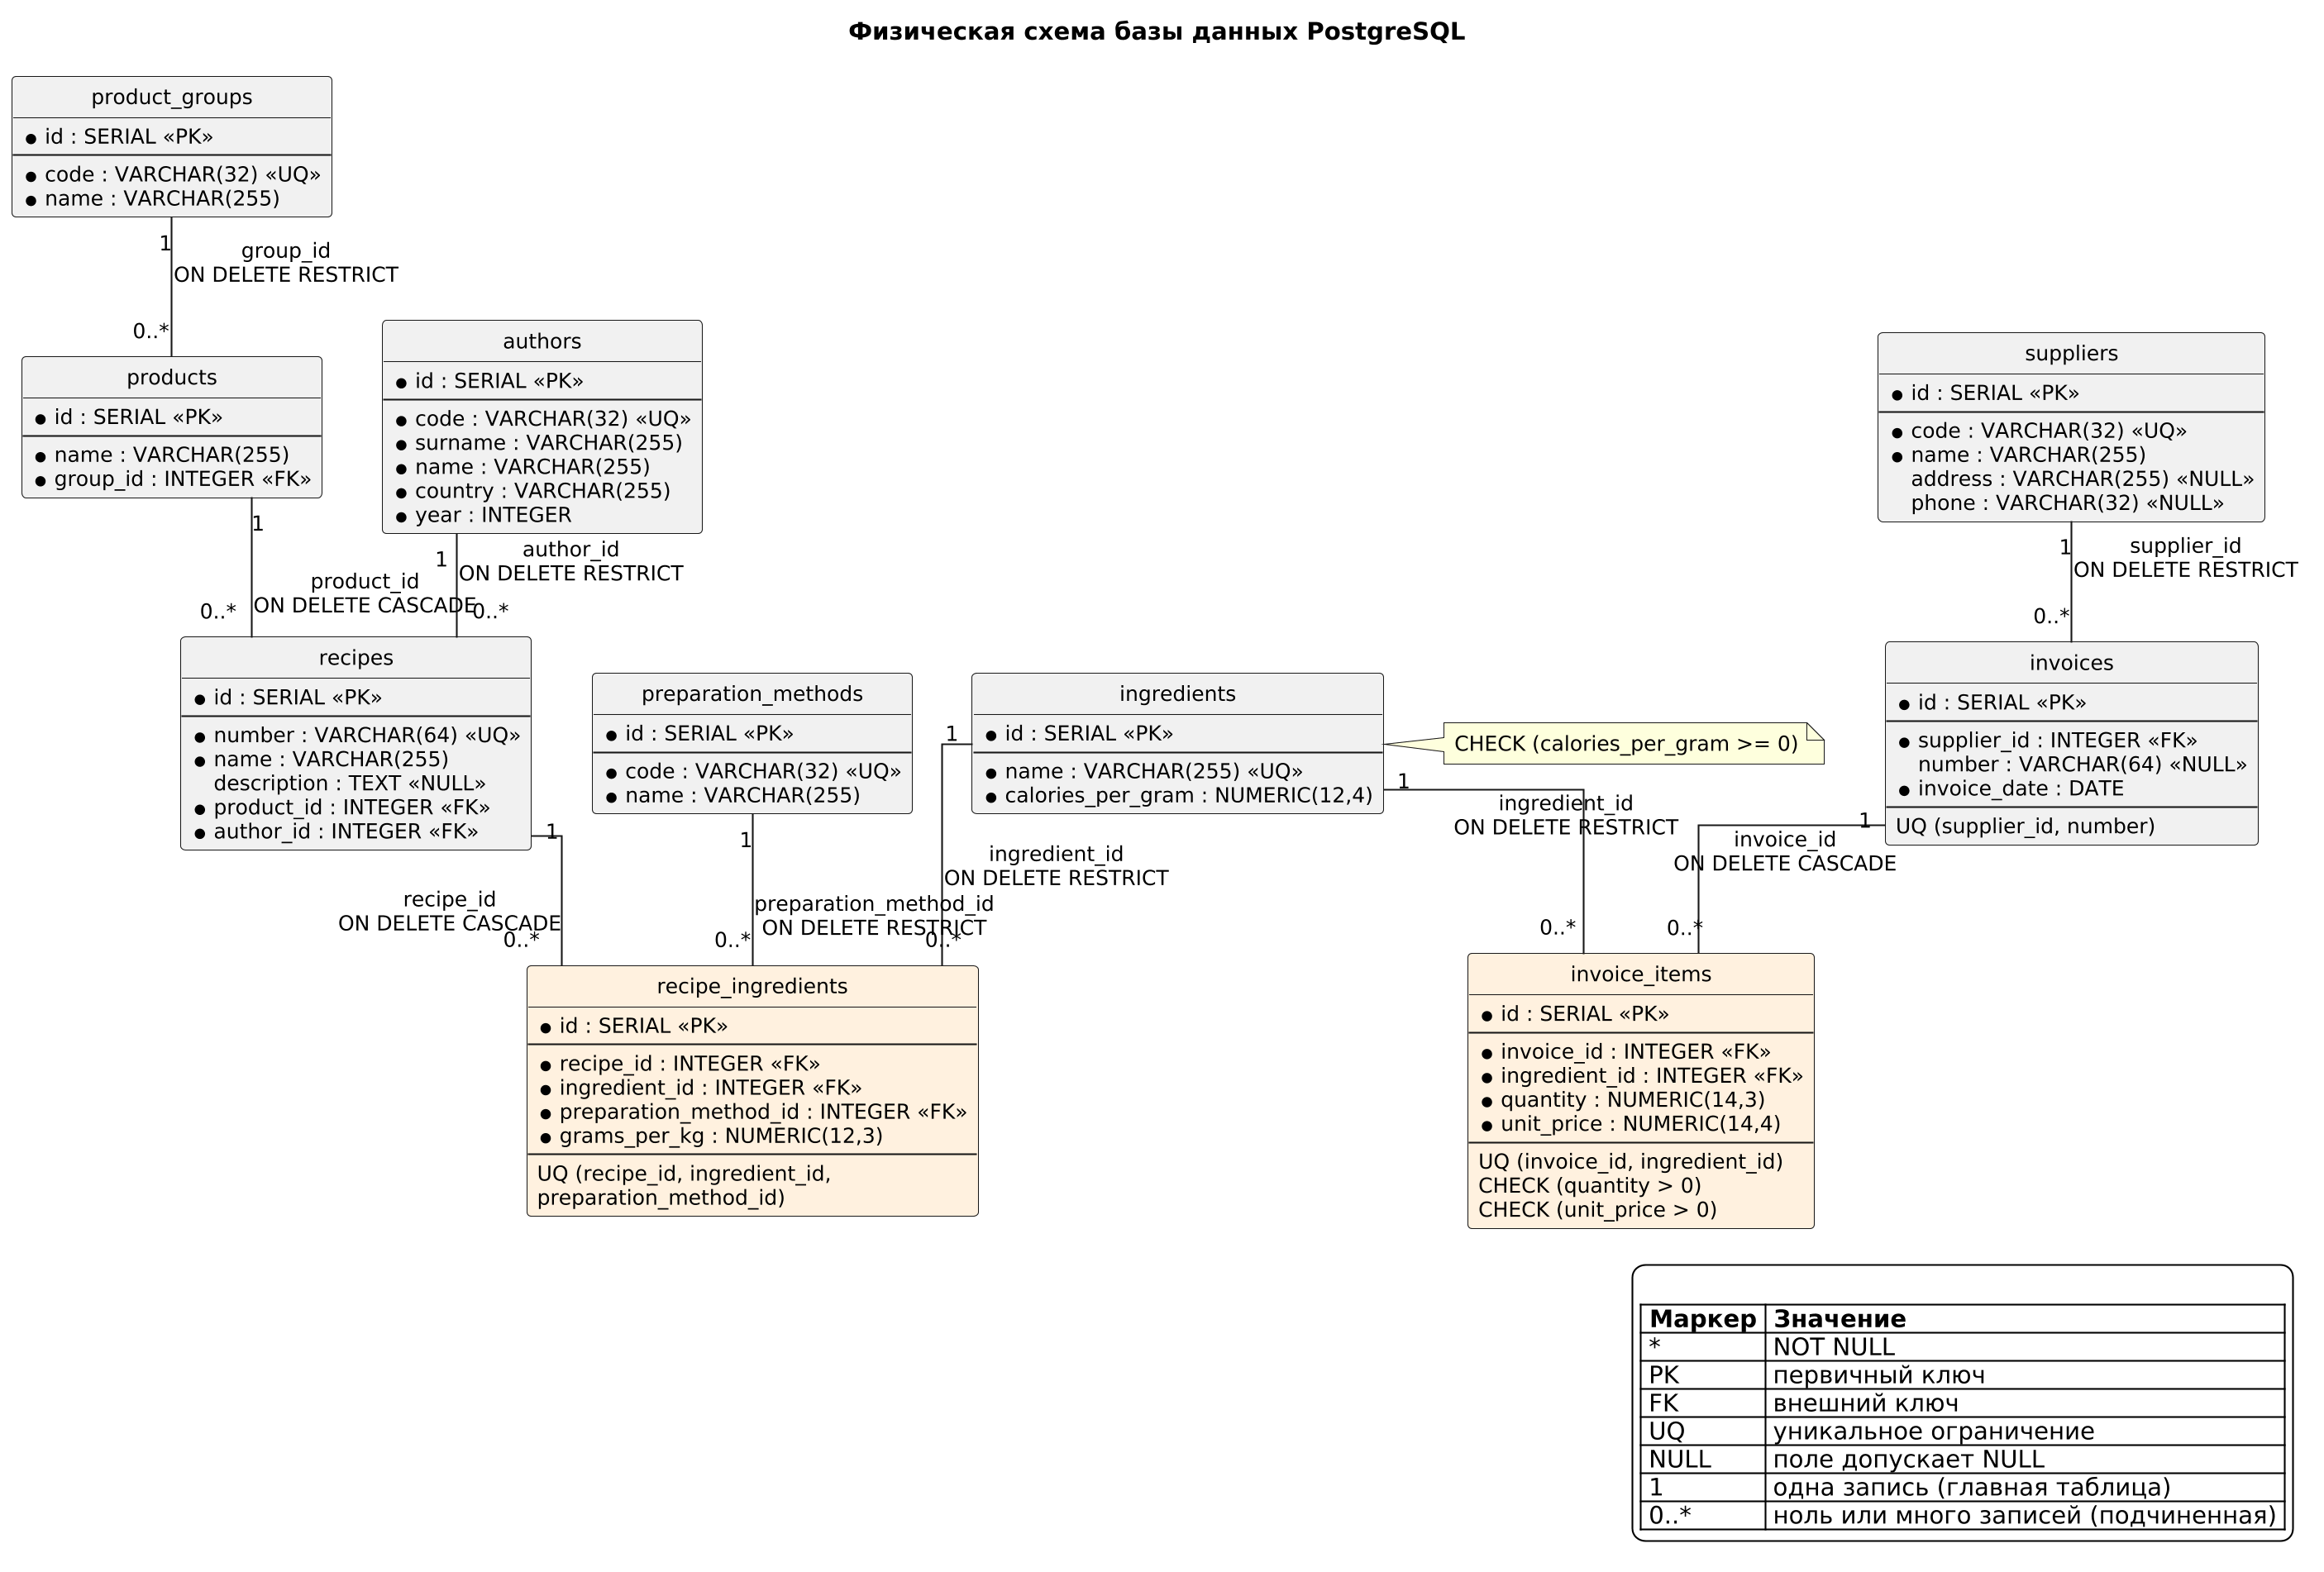
\includegraphics[width=0.99\linewidth,height=0.76\textheight,keepaspectratio]{images/03_physical_db.png}
\caption{Физическая схема базы данных PostgreSQL}
\label{fig:physical}
\end{figure}
\end{landscape}

Физическая модель ориентирована на PostgreSQL. Все таблицы имеют surrogate
primary key \texttt{id} типа \texttt{SERIAL}. Денежные, количественные и
калорийные значения хранятся в \texttt{NUMERIC}, чтобы исключить ошибки
двоичной арифметики с плавающей точкой. Схема представлена на
рисунке~\ref{fig:physical}.

\subsection{Ограничения и индексы}

На внешние ключи и дату накладной созданы индексы. Уникальные ограничения
защищают коды справочников, номер рецепта, пару «поставщик--номер накладной» и
повтор ингредиента внутри одной накладной. Ограничения \texttt{CHECK}
запрещают отрицательную калорийность, неположительные количество и цену.

Фрагмент физической схемы:

\begin{minted}{sql}
-- Позиция накладной не может существовать без накладной.
CREATE TABLE invoice_items (
    id            SERIAL PRIMARY KEY,
    invoice_id    INTEGER NOT NULL
                  REFERENCES invoices(id) ON DELETE CASCADE,
    ingredient_id INTEGER NOT NULL
                  REFERENCES ingredients(id) ON DELETE RESTRICT,
    quantity      NUMERIC(14, 3) NOT NULL,
    unit_price    NUMERIC(14, 4) NOT NULL,

    -- Один ингредиент встречается в накладной не более одного раза.
    CONSTRAINT uq_invoice_items_invoice_id_ingredient_id
        UNIQUE (invoice_id, ingredient_id),

    -- Некорректные количество и цена отвергаются самой СУБД.
    CONSTRAINT ck_invoice_items_quantity_positive CHECK (quantity > 0),
    CONSTRAINT ck_invoice_items_unit_price_positive CHECK (unit_price > 0)
);
\end{minted}

Начальное наполнение находится в \texttt{sql/02\_seed.sql}. Оно идемпотентно:
повторный запуск использует \texttt{ON CONFLICT DO NOTHING} и
\texttt{NOT EXISTS}, поэтому не создаёт дубликаты.

% ============================================================================
% 7. ОСНОВНЫЕ ЗАПРОСЫ, ФУНКЦИИ, ПРОЦЕДУРЫ И ТРИГГЕРЫ
% ============================================================================
\clearpage
\section{ОСНОВНЫЕ ЗАПРОСЫ, ФУНКЦИИ, ПРОЦЕДУРЫ И ТРИГГЕРЫ}

\subsection{Общий CRUD-запрос чтения}

SQLAlchemy используется для соединения и выполнения команд, но не для
генерации ORM-запросов. Значение \texttt{id} передаётся отдельно от SQL-текста,
что защищает запрос от SQL-инъекций.

\begin{minted}{python}
async def get(self, id: int) -> T | None:
    # Имена таблицы и столбцов заданы в серверном коде репозитория.
    # Пользователь не может передать их через HTTP.
    sql = text(
        f"SELECT id, {', '.join(self._columns)} "
        f"FROM {self._table} WHERE id = :id"
    )

    # Значение id отправляется драйверу как bind-параметр.
    row = (
        await self._session.execute(sql, {"id": id})
    ).mappings().one_or_none()

    return self._from_row(row) if row is not None else None
\end{minted}

\subsection{Создание записи}

Оператор \texttt{RETURNING} возвращает созданную строку и назначенный
PostgreSQL идентификатор без дополнительного \texttt{SELECT}.

\begin{minted}{sql}
-- name и group_id поступают из проверенной Pydantic-схемы,
-- но передаются в запрос только как параметры.
INSERT INTO products (name, group_id)
VALUES (:name, :group_id)
RETURNING id, name, group_id;
\end{minted}

После успешного выполнения репозиторий вызывает \texttt{commit}. При
\texttt{IntegrityError} выполняется \texttt{rollback}, а клиент получает HTTP
409.

\subsection{Чтение товара вместе с группой}

Запрос с \texttt{JOIN} используется вместо ORM-загрузки отношения. Псевдонимы
позволяют отличить поля товара от полей группы.

\begin{minted}{sql}
-- Возвращает товар и данные его группы одним запросом.
SELECT
    p.id,
    p.name,
    p.group_id,
    pg.id   AS group_object_id,
    pg.code AS group_code,
    pg.name AS group_name
FROM products AS p
JOIN product_groups AS pg ON pg.id = p.group_id
WHERE p.id = :id;
\end{minted}

\subsection{Прайс-лист поставщика}

Запрос выбирает цены только из накладных заданного поставщика за указанную
дату. Оба значения являются bind-параметрами.

\begin{minted}{sql}
-- Прайс-лист содержит ингредиент, цену и исходный номер накладной.
SELECT
    ing.id   AS ingredient_id,
    ing.name AS ingredient_name,
    ii.unit_price,
    inv.number AS invoice_number
FROM invoices AS inv
JOIN invoice_items AS ii ON ii.invoice_id = inv.id
JOIN ingredients AS ing ON ing.id = ii.ingredient_id
WHERE inv.supplier_id = :supplier_id
  AND inv.invoice_date = :price_date
ORDER BY ing.id, inv.id;
\end{minted}

\subsection{Расчёт минимальной калорийности}

Для каждого рецепта вычисляется калорийность одного килограмма:

\[
K_{1\,\text{кг}}=\sum_{i=1}^{n} k_i \cdot m_i,
\qquad
K_{100\,\text{г}}=\frac{K_{1\,\text{кг}}}{10}.
\]

CTE сначала агрегирует калорийность каждого рецепта, затем внешний запрос
выбирает все строки с минимальным значением.

\begin{minted}{sql}
-- Расчёт выполняется средствами PostgreSQL, а не циклом Python.
WITH recipe_calories AS (
    SELECT
        p.id AS product_id,
        p.name AS product_name,
        pg.name AS group_name,
        r.id AS recipe_id,
        r.name AS recipe_name,
        SUM(ing.calories_per_gram * ri.grams_per_kg)
            AS calories_per_1kg
    FROM recipes AS r
    JOIN products AS p ON p.id = r.product_id
    JOIN product_groups AS pg ON pg.id = p.group_id
    JOIN recipe_ingredients AS ri ON ri.recipe_id = r.id
    JOIN ingredients AS ing ON ing.id = ri.ingredient_id
    GROUP BY p.id, p.name, pg.name, r.id, r.name
)
SELECT *
FROM recipe_calories
WHERE calories_per_1kg = (
    SELECT MIN(calories_per_1kg)
    FROM recipe_calories
)
ORDER BY recipe_id;
\end{minted}

\subsection{Функции серверного приложения}

Прикладные функции реализованы асинхронными методами Python. Например,
\texttt{get\_session} управляет транзакцией на протяжении HTTP-запроса:

\begin{minted}{python}
async def get_session() -> AsyncGenerator[AsyncSession, None]:
    async with async_session_maker() as session:
        try:
            # Сессия передаётся endpoint через Depends.
            yield session
            await session.commit()
        except IntegrityError as exc:
            # При нарушении ограничений изменения отменяются.
            await session.rollback()
            raise exc
        except Exception:
            # Любая другая ошибка также не оставляет частичных изменений.
            await session.rollback()
            raise
\end{minted}

Функция dependency injection создаёт сервис с той же сессией:

\begin{minted}{python}
def get_product_service(
    session: Annotated[AsyncSession, Depends(get_session)],
) -> ProductService:
    # Endpoint получает готовый сервис и не управляет БД напрямую.
    return ProductService(session)
\end{minted}

\subsection{Generic-репозиторий}

Общий интерфейс параметризован типом сущности \texttt{T}. Поэтому один CRUD
алгоритм применяется к товарам, авторам, поставщикам и другим сущностям без
потери информации о возвращаемом типе.

\begin{minted}{python}
T = TypeVar("T", bound=Base)

class IRepository(ABC, Generic[T]):
    @abstractmethod
    async def get(self, id: int) -> T | None:
        raise NotImplementedError

    @abstractmethod
    async def list(
        self, *, offset: int = 0, limit: int = 100
    ) -> list[T]:
        raise NotImplementedError

class BaseRepository(IRepository[T], Generic[T]):
    # Реализует ручные SELECT, INSERT, UPDATE и DELETE.
    ...
\end{minted}

\subsection{Хранимые процедуры и триггеры}

В текущей версии базы данных пользовательские хранимые процедуры и триггеры
не применяются. Это осознанное архитектурное решение: CRUD и отчётная логика
сосредоточены в сервисах и репозиториях FastAPI, а PostgreSQL отвечает за
хранение, связи, проверки и агрегирование.

Функции, которые часто возлагаются на триггеры, реализованы декларативными
средствами БД:

\begin{itemize}[leftmargin=1.25cm]
    \item каскадное удаление --- внешними ключами \texttt{ON DELETE CASCADE};
    \item запрет удаления используемых справочников --- \texttt{ON DELETE RESTRICT};
    \item проверка положительных значений --- ограничениями \texttt{CHECK};
    \item предотвращение дублей --- ограничениями \texttt{UNIQUE};
    \item атомарность --- транзакциями \texttt{commit}/\texttt{rollback}.
\end{itemize}

Следовательно, текстов пользовательских \texttt{CREATE PROCEDURE},
\texttt{CREATE FUNCTION} и \texttt{CREATE TRIGGER} в проекте нет. Такой подход
не скрывает бизнес-логику внутри СУБД и делает её доступной для тестирования в
Python.

% ============================================================================
% 8. ИНТЕРФЕЙС ПРИЛОЖЕНИЯ
% ============================================================================
\clearpage
\section{ИНТЕРФЕЙС ПРИЛОЖЕНИЯ}

Frontend реализован в файле \texttt{static/index.html}. Сервер FastAPI отдаёт
его по корневому адресу \texttt{/}. Страница использует HTML, CSS и JavaScript
без отдельного frontend-фреймворка. Все данные загружаются через REST API с
префиксом \texttt{/api/v1}.

\subsection{Главное окно}

Главное окно содержит навигацию и таблицы основных сущностей: товаров,
рецептов, поставщиков, авторов, ингредиентов, групп товаров, способов
подготовки и накладных. После события \texttt{DOMContentLoaded} функция
\texttt{loadAllTables} вызывает API для каждого раздела. Полученный JSON
передаётся в универсальную функцию построения таблицы.

\optionalinterfacefigure{main_window}{Главное окно приложения}

\subsection{Окно создания записи}

Кнопка «Добавить» открывает модальное окно. Состав формы определяется объектом
\texttt{tableConfigs}: для каждого ресурса в нём заданы поля, подписи, типы и
признак обязательности. После подтверждения JavaScript отправляет
\texttt{POST}-запрос с JSON-телом. При успехе окно закрывается, а таблица
перезагружается.

\optionalinterfacefigure{create_window}{Окно создания записи}

\subsection{Окно изменения записи}

Перед редактированием frontend получает актуальную запись запросом
\texttt{GET /<resource>/<id>} и заполняет форму. Изменённые значения передаются
методом \texttt{PUT}. Не переданные необязательные поля сохраняют прежние
значения благодаря логике сервисного слоя.

\optionalinterfacefigure{edit_window}{Окно изменения записи}

\subsection{Интерактивная документация API}

FastAPI автоматически формирует Swagger UI по адресу \texttt{/docs}. В нём
можно просмотреть схемы Pydantic, параметры запросов, коды ответов и выполнить
любой endpoint без стороннего HTTP-клиента. Альтернативная документация ReDoc
доступна по адресу \texttt{/redoc}.

\optionalinterfacefigure{swagger}{Интерактивная документация Swagger UI}

\subsection{Обмен данными с сервером}

Универсальный вызов списка имеет следующий вид:

\begin{minted}{javascript}
// apiPath берётся из конфигурации выбранной таблицы.
const response = await fetch(
    `${API_BASE}${config.apiPath}/`
);

if (!response.ok) {
    throw new Error('Failed to fetch');
}

// Сервер возвращает JSON, из которого строится HTML-таблица.
const data = await response.json();
renderTable(tableName, data, config);
\end{minted}

% ============================================================================
% 9. ИНСТРУМЕНТАЛЬНЫЕ СРЕДСТВА
% ============================================================================
\clearpage
\section{ИНСТРУМЕНТАЛЬНЫЕ СРЕДСТВА}

\begin{longtable}{L{0.28\textwidth} L{0.62\textwidth}}
\toprule
\textbf{Средство} & \textbf{Назначение} \\
\midrule
\endhead
Python 3.11+ & Язык реализации серверной части и тестов. \\
FastAPI & Маршрутизация HTTP, dependency injection, обработка запросов и генерация OpenAPI. \\
Pydantic 2 & Валидация JSON и сериализация ответов. \\
PostgreSQL 17 & Реляционная СУБД, внешние ключи, ограничения, индексы, соединения и агрегирование. \\
SQLAlchemy 2 AsyncIO & Пул соединений, асинхронная сессия, транзакции и выполнение ручного SQL через \texttt{text}. \\
asyncpg & Асинхронный драйвер PostgreSQL. \\
HTML, CSS, JavaScript & Реализация web-интерфейса и обращение к API через \texttt{fetch}. \\
Docker Compose & Запуск PostgreSQL, постоянный volume и автоматическое подключение DDL/seed-скриптов. \\
pytest, pytest-asyncio & Модульные и интеграционные тесты асинхронного кода. \\
httpx & Проверка ASGI-приложения и PostgreSQL smoke-тест. \\
Ruff & Статический анализ и форматирование Python-кода. \\
Git & Контроль версий проекта. \\
MiKTeX, XeLaTeX & Подготовка и сборка отчёта. \\
\bottomrule
\end{longtable}

\subsection{Конфигурация и запуск}

Параметры соединения находятся в \texttt{.env} и читаются через
\texttt{pydantic-settings}. Пароль не зашит в исходный код. Docker Compose
подключает \texttt{sql/01\_schema.sql} и \texttt{sql/02\_seed.sql} как
инициализационные скрипты PostgreSQL.

\begin{minted}{text}
docker compose up -d
python -m uvicorn app.main:app --reload
\end{minted}

После запуска интерфейс доступен по адресу
\texttt{http://localhost:8000/}, Swagger UI --- по адресу
\texttt{http://localhost:8000/docs}.

\subsection{Тестирование}

Автоматические тесты проверяют CRUD, параметризацию SQL, работу с
\texttt{Decimal} и датами, загрузку связанных объектов и три отчётных запроса.
Строка, внешне похожая на SQL-инъекцию, сохраняется как обычное значение, что
подтверждает корректность bind-параметров.

Скрипт \texttt{scripts/smoke\_postgres.py} дополнительно проверяет полный
HTTP-цикл с реальной PostgreSQL: чтение коллекций, создание, получение,
обновление и удаление товара, а также запуск всех отчётов.

\clearpage
\section*{ЗАКЛЮЧЕНИЕ}
\addcontentsline{toc}{section}{Заключение}

В ходе лабораторной работы выполнено концептуальное, логическое и физическое
проектирование информационной системы для учёта технологий создания
продуктов. На концептуальном уровне определены актор, варианты использования
и сценарии взаимодействия. Логическая модель описывает сущности и мощности
связей, а физическая схема задаёт таблицы PostgreSQL, типы, ключи, индексы и
ограничения целостности.

На основе спроектированной базы разработано асинхронное web-приложение.
Frontend взаимодействует с REST API, сервер разделён на контроллеры, сервисы и
репозитории. Все запросы написаны вручную и используют bind-параметры.
Generic-репозиторий уменьшает дублирование CRUD-кода, а Pydantic и ограничения
PostgreSQL обеспечивают многоуровневую проверку данных.

Работоспособность подтверждена модульными тестами и smoke-тестом на реальной
PostgreSQL. Разработанная структура допускает добавление новых справочников,
отчётов и интерфейсных представлений без изменения базовых принципов системы.

\clearpage
\section*{СПИСОК ИСПОЛЬЗОВАННЫХ ИСТОЧНИКОВ}
\addcontentsline{toc}{section}{Список использованных источников}

\begin{enumerate}[label={\lbrack\arabic*\rbrack}]
    \item PostgreSQL 17 Documentation. --- \url{https://www.postgresql.org/docs/17/}.
    \item FastAPI Documentation. --- \url{https://fastapi.tiangolo.com/}.
    \item SQLAlchemy 2.0 Documentation. --- \url{https://docs.sqlalchemy.org/en/20/}.
    \item Pydantic Documentation. --- \url{https://docs.pydantic.dev/latest/}.
    \item Docker Compose Documentation. --- \url{https://docs.docker.com/compose/}.
    \item Object Management Group. Unified Modeling Language. --- \url{https://www.omg.org/spec/UML/}.
\end{enumerate}

\end{document}
